\documentclass[]{elsarticle} %review=doublespace preprint=single 5p=2 column
%%% Begin My package additions %%%%%%%%%%%%%%%%%%%
\usepackage[hyphens]{url}

  \journal{Journal of Hydrology} % Sets Journal name


\usepackage{lineno} % add
  \linenumbers % turns line numbering on
\providecommand{\tightlist}{%
  \setlength{\itemsep}{0pt}\setlength{\parskip}{0pt}}

\usepackage{graphicx}
\usepackage{booktabs} % book-quality tables
%%%%%%%%%%%%%%%% end my additions to header

\usepackage[T1]{fontenc}
\usepackage{lmodern}
\usepackage{amssymb,amsmath}
\usepackage{ifxetex,ifluatex}
\usepackage{fixltx2e} % provides \textsubscript
% use upquote if available, for straight quotes in verbatim environments
\IfFileExists{upquote.sty}{\usepackage{upquote}}{}
\ifnum 0\ifxetex 1\fi\ifluatex 1\fi=0 % if pdftex
  \usepackage[utf8]{inputenc}
\else % if luatex or xelatex
  \usepackage{fontspec}
  \ifxetex
    \usepackage{xltxtra,xunicode}
  \fi
  \defaultfontfeatures{Mapping=tex-text,Scale=MatchLowercase}
  \newcommand{\euro}{€}
\fi
% use microtype if available
\IfFileExists{microtype.sty}{\usepackage{microtype}}{}
\bibliographystyle{elsarticle-harv}
\usepackage{color}
\usepackage{fancyvrb}
\newcommand{\VerbBar}{|}
\newcommand{\VERB}{\Verb[commandchars=\\\{\}]}
\DefineVerbatimEnvironment{Highlighting}{Verbatim}{commandchars=\\\{\}}
% Add ',fontsize=\small' for more characters per line
\usepackage{framed}
\definecolor{shadecolor}{RGB}{248,248,248}
\newenvironment{Shaded}{\begin{snugshade}}{\end{snugshade}}
\newcommand{\AlertTok}[1]{\textcolor[rgb]{0.94,0.16,0.16}{#1}}
\newcommand{\AnnotationTok}[1]{\textcolor[rgb]{0.56,0.35,0.01}{\textbf{\textit{#1}}}}
\newcommand{\AttributeTok}[1]{\textcolor[rgb]{0.77,0.63,0.00}{#1}}
\newcommand{\BaseNTok}[1]{\textcolor[rgb]{0.00,0.00,0.81}{#1}}
\newcommand{\BuiltInTok}[1]{#1}
\newcommand{\CharTok}[1]{\textcolor[rgb]{0.31,0.60,0.02}{#1}}
\newcommand{\CommentTok}[1]{\textcolor[rgb]{0.56,0.35,0.01}{\textit{#1}}}
\newcommand{\CommentVarTok}[1]{\textcolor[rgb]{0.56,0.35,0.01}{\textbf{\textit{#1}}}}
\newcommand{\ConstantTok}[1]{\textcolor[rgb]{0.00,0.00,0.00}{#1}}
\newcommand{\ControlFlowTok}[1]{\textcolor[rgb]{0.13,0.29,0.53}{\textbf{#1}}}
\newcommand{\DataTypeTok}[1]{\textcolor[rgb]{0.13,0.29,0.53}{#1}}
\newcommand{\DecValTok}[1]{\textcolor[rgb]{0.00,0.00,0.81}{#1}}
\newcommand{\DocumentationTok}[1]{\textcolor[rgb]{0.56,0.35,0.01}{\textbf{\textit{#1}}}}
\newcommand{\ErrorTok}[1]{\textcolor[rgb]{0.64,0.00,0.00}{\textbf{#1}}}
\newcommand{\ExtensionTok}[1]{#1}
\newcommand{\FloatTok}[1]{\textcolor[rgb]{0.00,0.00,0.81}{#1}}
\newcommand{\FunctionTok}[1]{\textcolor[rgb]{0.00,0.00,0.00}{#1}}
\newcommand{\ImportTok}[1]{#1}
\newcommand{\InformationTok}[1]{\textcolor[rgb]{0.56,0.35,0.01}{\textbf{\textit{#1}}}}
\newcommand{\KeywordTok}[1]{\textcolor[rgb]{0.13,0.29,0.53}{\textbf{#1}}}
\newcommand{\NormalTok}[1]{#1}
\newcommand{\OperatorTok}[1]{\textcolor[rgb]{0.81,0.36,0.00}{\textbf{#1}}}
\newcommand{\OtherTok}[1]{\textcolor[rgb]{0.56,0.35,0.01}{#1}}
\newcommand{\PreprocessorTok}[1]{\textcolor[rgb]{0.56,0.35,0.01}{\textit{#1}}}
\newcommand{\RegionMarkerTok}[1]{#1}
\newcommand{\SpecialCharTok}[1]{\textcolor[rgb]{0.00,0.00,0.00}{#1}}
\newcommand{\SpecialStringTok}[1]{\textcolor[rgb]{0.31,0.60,0.02}{#1}}
\newcommand{\StringTok}[1]{\textcolor[rgb]{0.31,0.60,0.02}{#1}}
\newcommand{\VariableTok}[1]{\textcolor[rgb]{0.00,0.00,0.00}{#1}}
\newcommand{\VerbatimStringTok}[1]{\textcolor[rgb]{0.31,0.60,0.02}{#1}}
\newcommand{\WarningTok}[1]{\textcolor[rgb]{0.56,0.35,0.01}{\textbf{\textit{#1}}}}
\usepackage{longtable}
\usepackage{graphicx}
\ifxetex
  \usepackage[setpagesize=false, % page size defined by xetex
              unicode=false, % unicode breaks when used with xetex
              xetex]{hyperref}
\else
  \usepackage[unicode=true]{hyperref}
\fi
\hypersetup{breaklinks=true,
            bookmarks=true,
            pdfauthor={},
            pdftitle={Do larger catchments respond different to forest cover change? Re-analysing a global data set.},
            colorlinks=false,
            urlcolor=blue,
            linkcolor=magenta,
            pdfborder={0 0 0}}
\urlstyle{same}  % don't use monospace font for urls

\setcounter{secnumdepth}{0}
% Pandoc toggle for numbering sections (defaults to be off)
\setcounter{secnumdepth}{0}

% Pandoc citation processing

% Pandoc header



\begin{document}
\begin{frontmatter}

  \title{Do larger catchments respond different to forest cover change?
Re-analysing a global data set.}
    \author[The University of Sydney, INIA]{R. Willem Vervoort\corref{1}}
   \ead{willem.vervoort@sydney.edu.au} 
    \author[INIA]{Eliana Nervi}
   \ead{eliananervi@gmail.com} 
    \author[IMFIA]{Jimena Alonso\corref{2}}
   \ead{jalonso@fing.edu.uy} 
      \address[The University of Sydney]{School of Life and Environmental Sciences, The University of Sydney,
Sydney, NSW 2006, Australia}
    \address[INIA]{INIA, Uruguay}
    \address[IMFIA]{Institute of Fluid Mechanics and Environmental Engineering, School of
Engineering, Universidad de la República, 11200 Montevideo, Departamento
de Montevideo, Uruguay}
      \cortext[1]{Corresponding Author}
    \cortext[2]{Equal contribution}
  
  \begin{abstract}
  This is the abstract.
  
  It consists of two paragraphs.
  \end{abstract}
  
 \end{frontmatter}

\hypertarget{introduction}{%
\section{Introduction}\label{introduction}}

\hypertarget{introduction-1}{%
\subsection{Introduction}\label{introduction-1}}

There has been an long and on-going discussion in the hydrologcal
literature around the impact of forests on streamflow (Andréassian,
2004; Brown et al., 2013, 2005; Filoso et al., 2017; Jackson et al.,
2005; Zhang et al., 2017). The historic work highlights a general
consensus that if forest areas increase, streamflow decreases and
vice-versa. The most dramatic result in relation to this, is Figure 5 in
Zhang et al. (2011) indicating (for Australian watersheds) a 100\%
decrease in stream flow for watersheds with 100\% forest cover. However,
on the other end of the spectrum, in a series of French watersheds
(Cosandey et al., 2005), there was no change in streamflow
characteristics in 2 of the three watersheds studied in relation to
deforestation.

Several review papers have summarized different studies across the
globe, in relation to paired watershed studies (Bosch and Hewlett, 1982;
Brown et al., 2005), related to reforestation in particular (Filoso et
al., 2017), and more generally (Jackson et al., 2005; Zhang et al.,
2017). These studies aim to generalize the individual findings and to
identify if there are global trends or relationships that can be
developed. The most recent reviews (Filoso et al., 2017; Zhang et al.,
2017) developed an impressive global database of watershed studies in
relation to changes in streamflow due to changes in forest cover. The
Zhang et al. (2017) dataset, which covers over 250 studies, is described
in terms of the change in streamflow as a result of the change in forest
cover, where studies related to both forestation (increase in forest
cover) and deforestation (decrease in forest cover) were included. In
contrast, the paper by Filoso et al. (2017) focused primarily on
reforestation, and covered an equally impressive database of 167 studies
using a systematic review. In this case the collected data is mostly
coded as count data and only a subset of 37 studies was analysed for
actual water yield change.

The conclusions of the first paper (Zhang et al., 2017) suggest that
there is a distinct difference in the change in flow as a result of
forestation or deforestation between small watersheds, defined as
\textless{} 1000 km\textsuperscript{2} and large watersheds
\textgreater{} 1000 km\textsuperscript{2}. While for small watersheds
there was no real change in runoff with changes in cover, for large
watersheds there was a clear trend showing a decrease in runoff with and
increase in forest cover. Their main conclusion was that the response in
annual runoff to forest cover was scale dependent and appeared to be
more sensitive to forest cover change in water limited watersheds
relative to energy limited watershed (Zhang et al., 2017).

The second study (Filoso et al., 2017) was a systematic review which
classified the historical research and highlighted gaps in the spatial
distribution, the types of studies and the types of analysis. Their main
conclusion was also that reforestation decreases streamflow, but that
there were many interacting factors. For a subset of quantitative data
(37) they showed a relationship between catchment size and decline in
streamflow.

A final summary paper that includes much of the same data as Zhang et
al. (2017) and Filoso et al. (2017) is Zhou et al. (2015), which has one
author in common with Zhang et al. (2017). However, this paper aims to
explain the variation in the data using the Fuh model, and in particular
aims to link the variation in the observed data to variations in the
exponent \emph{m} in the model. A key observation is that in drier
environments, the effects of deforestation are much greater than in
wetter environments, which is also suggested by Figure 4 in Zhang et al.
(2017).

Encouraged by the work presented by Zhang et al. (2017) and Filoso et
al. (2017) and the fantastic database of studies presented by these
authors, we believe we can add to the discussion. In this paper, the aim
is to develop further analysis of the collected data and expanding and
combining the two data sets to provide further depth.

In particular, the main method in the work by Zhang et al. (2017) is
using simple linear regression, and in Filoso et al. (2017) the focus is
mainly on classification. As Zhang et al. (2017) points out, the main
assumption in their work is that the threshold at 1000
km\textsuperscript{2} is a distinct separation between ``small'' and
``large'' watersheds, but the subset of data in Filoso et al. (2017)
does not appear to support this. And while te work Filoso et al. (2017)
provides important insights in study types, analysis types and broad
classification, there is limited quantification of actual impact. This
is because the work had a strict criterion to select quantitative
studies. However, given the fantastic data sets collected, the analyses
can be easily expanded to look at interactions between the terms and to
test the assumption of a distinct threshold at 1000
km\textsuperscript{2}.

As a result the objective of this paper is to 1) enhance the data set
from Zhang et al. (2017) with further watersheds (such as from Filoso et
al. (2017)) and spatial coordinates and 2) to analyse the possibility of
non-linear, interactions and partial effects of the different factors
and variables in the data using generalised linear (GLM) and generalised
additive models (GAM Wood (2006)).

Building on the analyses by Zhang et al. (2017) and Filoso et al.
(2017), and combining their conclusions, the main hypothesis to test is
that the change in streamflow is impacted by the change in forest cover.
However, this change is clearly modulated by the area under
consideration (affecting the length of the flowpaths Zhou et al.
(2015)), the length of the study (c.f. Jackson et al. (2005)) and
possibly the climate (as indicated by either E0/Pa or latitude and
longitude Filoso et al. (2017); Zhou et al. (2015)).

However, there could be further confounding factors, which are eluded to
by Filoso et al. (2017):

\begin{itemize}
\item
  the type of analysis, i.e.~paired catchment studies, modelling, time
  series analysis etc.
\item
  the age of the study, assuming that historical studies might not have
  had the ability to measure at the accuracy that currently is available
  to researchers, or that more careful historical attention to detail in
  field studies might have been lost more recently due to reductions in
  research investment.
\end{itemize}

Finally, this work aims to point to further research that can expand
this area of work, based on the collected data, to better understand the
impact of forest cover change on streamflow.

\hypertarget{methods}{%
\section{Methods}\label{methods}}

\hypertarget{the-original-data-sets}{%
\subsection{The original data sets}\label{the-original-data-sets}}

The starting point of this paper is the data base of studies which were
included in Zhang et al. (2017) as supplementary material. The columns
in this data set are the watershed number, the watershed name, the Area
in km\textsuperscript{2}, the annual average precipitation (Pa) in mm,
the forest type, hydrological regime, and climate type, the change in
forest cover in \% (\(\Delta\)F\%) and the change in streamflow in \%
(\(\Delta\)Qf(\%), based on equation 1 in Zhang et al. (2017)), the
precipitation data type, the assessment technique, and the source of the
info, which is a citation. Several of these columns contain
abbreviations to describe the different variables, which are summarised
in Table 1.

Table 1 Summary of abbreviations of factors used in the Zhang et al.
(2017) data set

\begin{longtable}[]{@{}lll@{}}
\toprule
Factor & Abbreviation & Definition\tabularnewline
\midrule
\endhead
forest type & CF & coniferous forest\tabularnewline
& BF & broadleaf forest\tabularnewline
& MF & mixed forest\tabularnewline
hydrological regime & RD & rain dominated\tabularnewline
& SD & snow dominated\tabularnewline
climate type & EL & energy limited\tabularnewline
& WL & water limited\tabularnewline
& EQ & equitant\tabularnewline
precipitation data type & OB & observed\tabularnewline
& SG & spatial gridded\tabularnewline
& MD & modelled\tabularnewline
assessment technique & PWE & paired watershed experiment\tabularnewline
& QPW & quasi-paired watershed experiment\tabularnewline
& HM & hydrological modelling\tabularnewline
& EA & elastictity analysis\tabularnewline
& SH & combined use of statistical methods\tabularnewline
& & and hydrographs\tabularnewline
\bottomrule
\end{longtable}

While Zhang et al. (2017) use the dryness index in their analysis,
potential or reference evapotranspiration was not originally included as
part of the published data set. We combined the tables for small
(\textless{} 1000 km\textsuperscript{2}) and large (\textgreater= 1000
km\textsuperscript{2}) watershed data sets in our analysis.

\hypertarget{additional-data-collection}{%
\subsection{Additional data
collection}\label{additional-data-collection}}

To enhance the existing data set, this study added additional variables
and cross-checked the studies with the data set from Filoso et al.
(2017). In particular, we focussed on the 37 data points included in the
quantitative analysis in Filoso et al. (2017).

In addition, additional variables added were the latitude and longitude
for the center of the watershed as an approximation of its spatial
location. Using this information annual average reference
evapotranspiration (E0) was extracted from \textbf{XXXXX} if a value of
E0 was not available from the original papers. For large watersheds,
this value, similar to annual average rainfall, is only an approximation
of the climate at the location.

The length of the study can be a variable influencing the change in flow
(e.g.~Jackson et al., 2005) and therefore, the length, starting data and
completion date of the different studies was extracted from the
references provided by Zhang et al. (2017).

Several additional data points from watershed studies were extracted
from Zhang et al. (2011), Zhao et al. (2010), Borg et al. (1988),
Thornton et al. (2007), Zhou et al. (2010), Rodriguez et al. (2010),
Ruprecht et al. (1991) and Peña-Arancibia et al. (2012), and these were
checked against the existing studies to prevent overlap. In the citation
column in the data set, in general the main reference for the calculated
change in streamflow was used, because sometimes the original study did
not provide the quantification of the change in streamflow (i.e.~Table 6
in Zhang et al. (2011))

The final column in the improved data set is a ``notes'' column, which
is not further used in the analysis, but gives context to some of the
data for future research and highlights some of the discrepancies that
we found between the original papers and the data in the tables from
Zhang et al. (2017).

\hypertarget{statistical-modelling}{%
\subsection{Statistical modelling}\label{statistical-modelling}}

\begin{verbatim}
## Warning: NAs introduced by coercion

## Warning: NAs introduced by coercion
\end{verbatim}

To estimate how the change in streamflow is affected by the change in
forest cover while considering the effects of the other variables, we
applied generalised additive modelling (GAM) (Wood, 2006).

The first model applied in this analysis is based on the main hypothesis
outlined above, can the change in streamflow be predicted from the
change in forest cover, modulated by area, the length of the study and
the climate.

\[\tag{1}
\begin{aligned}
\Delta \%Q \sim ~&\Delta \%forest + Pa + Area + Latitude + Longitude + \varepsilon
\end{aligned}\]

However, the overall skewed distribution of the predictant
(\(\Delta \%Q\)) is problematic, and this results in a skewed
distribution of the GAM model residuals, which violates the linear model
assumptions. As a result we transformed \(\Delta \%Q\) back to fractions
(0 - 1) and log transformed using \(log10(x + 1)\), where \(x\) is
\(\Delta Q\). After transformation the model residuals approximate
\(\sim N(0,\sigma^2)\) and this results in the following equation:

\[\tag{2}
\begin{aligned}
log10(\frac{\Delta \% Q}{100} + 1) \sim ~ &\Delta \%{forest~cover}
+ Pa + Area + Latitude + 
\\ &Longitude + \varepsilon
\end{aligned}\]

A second model included all the variables in the analysis from Zhang et
al. (2017) in one model:

\[\tag{3}
\begin{aligned}
log10(\frac{\Delta \% Q}{100} + 1) \sim ~ &\Delta \% forest~cover + s(Pa, k = 3) + s(Area, k = 3) +  \\
& {forest~type} + {climate~type} + {assessment~type} + \\  
& {hydrologic~regime} + \varepsilon
\end{aligned}\]

In this model, no direct interactions are assumed, and the assumption is
that all continuous variables (such as Pa) can have a linear or
non-linear relationship with \(log10(\Delta Q)\). This means that a
smooth function \(s()\) is applied to the variable. To restrict the
smoothness of the fit, the smoothness factor \(k\) is restricted to a
value of 3 (Wood, 2006). This restriction was applied to smooth
variables throughout this paper and we have dropped this from the
notation in subsequent equations.

For the model in equation 3, we only used the data from Zhang et al.
(2017) to make sure that the additional watersheds added to the data set
did not influence the analysis. Given that in Zhang et al. (2017),
dryness (\(\frac{E0}{Pa}\)) is used to look at variations in the change
in flow, we also fitted the following model:

\[\tag{4}
\begin{aligned}
log10(\frac{\Delta \% Q}{100} + 1) \sim ~&\Delta \% forest~cover + s(\frac{E0}{Pa}) + s(Area) +  {forest~type} + 
\\  &{climate~type} + {assessment~type} + \\  &{hydrologic~regime} + \varepsilon
\end{aligned}\]

Subsequently, using the full data set, including the additional
watersheds and the additional variables the following two models were
fitted:

\[\tag{5}
\begin{aligned}
log10(\frac{\Delta \% Q}{100} + 1) \sim ~&\Delta \% forest~cover + s(Pa) + s(Area) + s(Latitude) + \\
& s(Longitude) + s(begin_{year}) + s(length_{study}) +\\
&{forest~type} + {climate~type} + {assessment~type} +\\
& {hydrologic~regime} + \varepsilon
\end{aligned}\]

\[\tag{6}
\begin{aligned}
log10(\frac{\Delta \% Q}{100} + 1) \sim ~&\Delta \% forest~cover +
s(\frac{E0}{Pa}) + s(Area) + \\ 
& s(Latitude) + s(Longitude) + s(begin_{year}) + \\ 
& s(length_{study}) + {forest~type} + {climate~type} + \\ 
& {assessment~type} + {hydrologic~regime} + \varepsilon
\end{aligned}\]

\hypertarget{results}{%
\section{Results}\label{results}}

\begin{verbatim}
## Loading required package: mgcv
\end{verbatim}

\begin{verbatim}
## Loading required package: nlme
\end{verbatim}

\begin{verbatim}
## 
## Attaching package: 'nlme'
\end{verbatim}

\begin{verbatim}
## The following object is masked from 'package:dplyr':
## 
##     collapse
\end{verbatim}

\begin{verbatim}
## This is mgcv 1.8-35. For overview type 'help("mgcv-package")'.
\end{verbatim}

\begin{verbatim}
## Warning in eval(predvars, data, env): NaNs produced

## Warning in eval(predvars, data, env): NaNs produced
\end{verbatim}

\begin{verbatim}
## 
## Family: gaussian 
## Link function: identity 
## 
## Formula:
## log10(DeltaQf_perc/100 + 1) ~ DeltaF_perc + Area_km2 + Pa_mm
## 
## Parametric coefficients:
##               Estimate Std. Error t value Pr(>|t|)    
## (Intercept)  4.430e-02  1.759e-02   2.519   0.0123 *  
## DeltaF_perc -1.345e-03  1.468e-04  -9.163   <2e-16 ***
## Area_km2    -1.657e-08  3.057e-08  -0.542   0.5883    
## Pa_mm       -7.989e-06  1.164e-05  -0.686   0.4930    
## ---
## Signif. codes:  0 '***' 0.001 '**' 0.01 '*' 0.05 '.' 0.1 ' ' 1
## 
## 
## R-sq.(adj) =   0.21   Deviance explained = 21.8%
## GCV = 0.018116  Scale est. = 0.017882  n = 310
\end{verbatim}

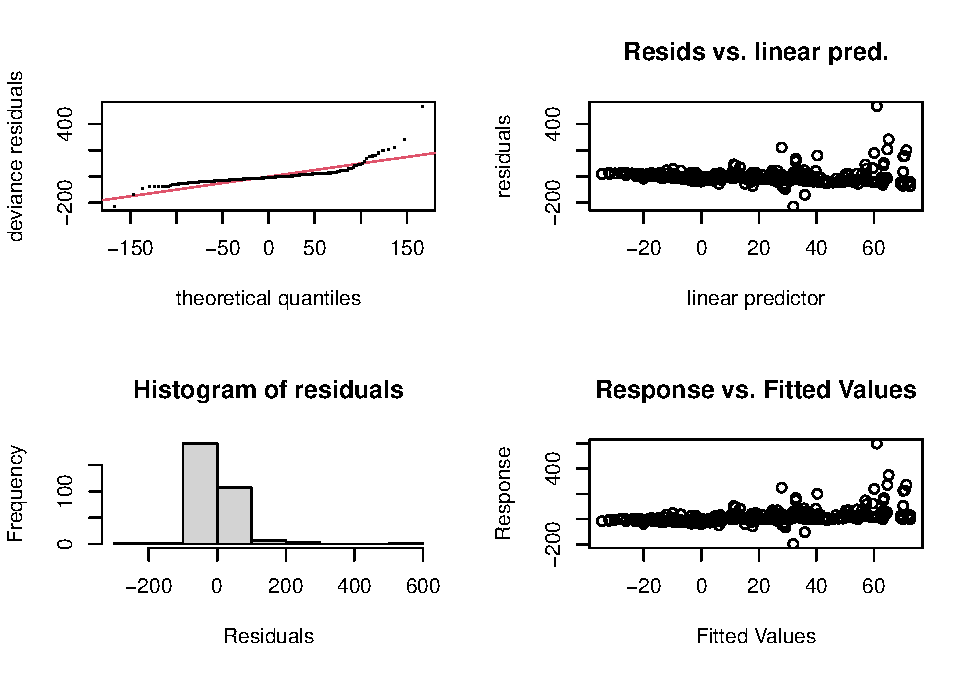
\includegraphics{Forest_and_Water_files/figure-latex/model2-1.pdf}

\begin{verbatim}
## 
## Method: GCV   Optimizer: magic
## Model required no smoothing parameter selectionModel rank =  4 / 4
\end{verbatim}

\begin{verbatim}
## Warning in eval(predvars, data, env): NaNs produced

## Warning in eval(predvars, data, env): NaNs produced
\end{verbatim}

\begin{verbatim}
## 
## Family: gaussian 
## Link function: identity 
## 
## Formula:
## log10(DeltaQf_perc/100 + 1) ~ DeltaF_perc + Area_km2 + Pa_mm + 
##     Latitude + Longitude
## 
## Parametric coefficients:
##               Estimate Std. Error t value Pr(>|t|)    
## (Intercept)  7.296e-02  1.964e-02   3.715 0.000243 ***
## DeltaF_perc -1.552e-03  1.526e-04 -10.173  < 2e-16 ***
## Area_km2    -2.963e-08  2.996e-08  -0.989 0.323525    
## Pa_mm       -1.382e-05  1.205e-05  -1.147 0.252393    
## Latitude    -1.276e-03  2.826e-04  -4.516 9.07e-06 ***
## Longitude   -2.121e-05  8.975e-05  -0.236 0.813323    
## ---
## Signif. codes:  0 '***' 0.001 '**' 0.01 '*' 0.05 '.' 0.1 ' ' 1
## 
## 
## R-sq.(adj) =  0.271   Deviance explained = 28.3%
## GCV = 0.017125  Scale est. = 0.016787  n = 304
\end{verbatim}

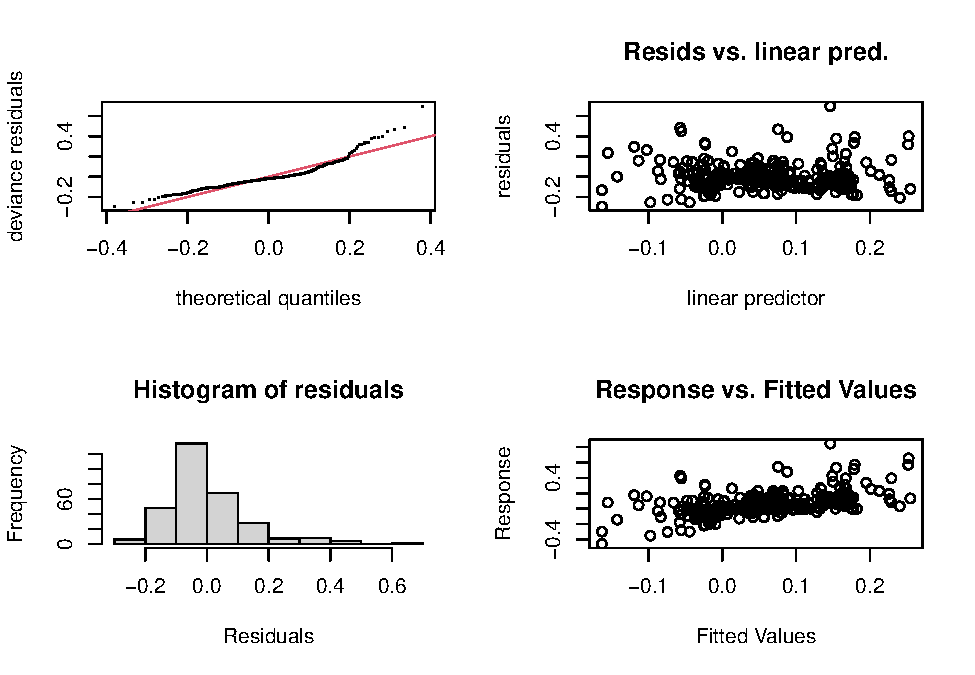
\includegraphics{Forest_and_Water_files/figure-latex/model2a-1.pdf}

\begin{verbatim}
## 
## Method: GCV   Optimizer: magic
## Model required no smoothing parameter selectionModel rank =  6 / 6
\end{verbatim}

\begin{verbatim}
## Warning in eval(predvars, data, env): NaNs produced

## Warning in eval(predvars, data, env): NaNs produced
\end{verbatim}

\begin{verbatim}
## 
## Family: gaussian 
## Link function: identity 
## 
## Formula:
## log10(DeltaQf_perc/100 + 1) ~ DeltaF_perc + log10(Area_km2) + 
##     Pa_mm + Latitude + Longitude + From + length
## 
## Parametric coefficients:
##                   Estimate Std. Error t value Pr(>|t|)    
## (Intercept)     -1.027e+00  9.040e-01  -1.136 0.256902    
## DeltaF_perc     -1.267e-03  1.594e-04  -7.947 5.83e-14 ***
## log10(Area_km2) -2.003e-02  4.386e-03  -4.567 7.63e-06 ***
## Pa_mm           -7.871e-06  1.255e-05  -0.627 0.531281    
## Latitude        -1.084e-03  2.834e-04  -3.827 0.000163 ***
## Longitude        6.268e-05  9.560e-05   0.656 0.512595    
## From             5.612e-04  4.583e-04   1.225 0.221809    
## length          -2.931e-06  7.036e-06  -0.417 0.677294    
## ---
## Signif. codes:  0 '***' 0.001 '**' 0.01 '*' 0.05 '.' 0.1 ' ' 1
## 
## 
## R-sq.(adj) =  0.303   Deviance explained = 32.1%
## GCV = 0.016008  Scale est. = 0.01553   n = 268
\end{verbatim}

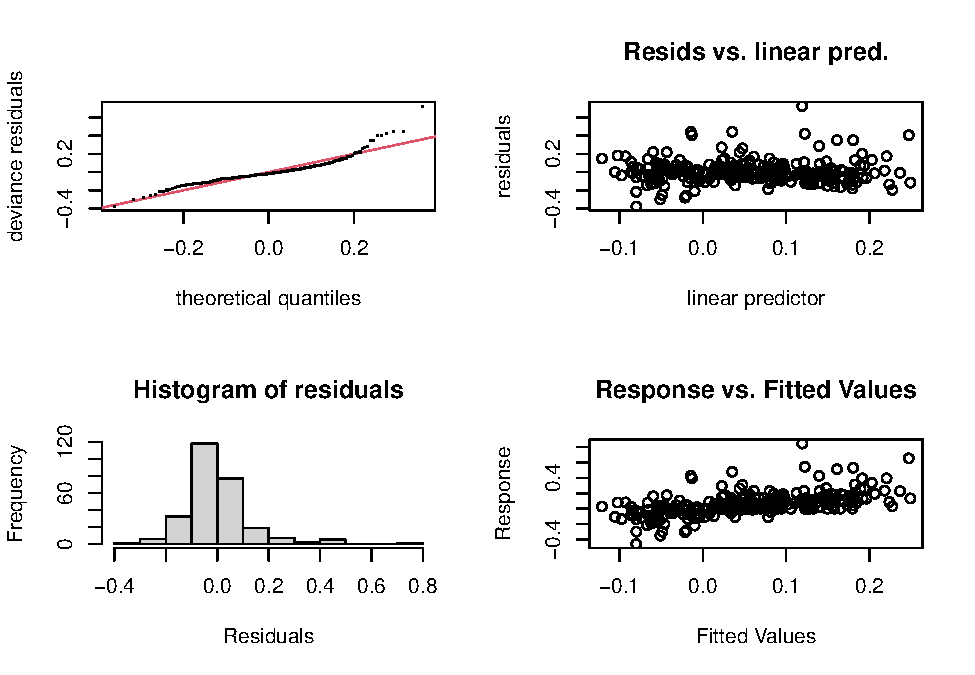
\includegraphics{Forest_and_Water_files/figure-latex/model2a1-1.pdf}

\begin{verbatim}
## 
## Method: GCV   Optimizer: magic
## Model required no smoothing parameter selectionModel rank =  8 / 8
\end{verbatim}

\begin{verbatim}
## Warning in eval(predvars, data, env): NaNs produced

## Warning in eval(predvars, data, env): NaNs produced
\end{verbatim}

\begin{verbatim}
## 
## Family: gaussian 
## Link function: identity 
## 
## Formula:
## log10(DeltaQf_perc/100 + 1) ~ DeltaF_perc + s(Area_km2, k = 3) + 
##     s(Pa_mm, k = 3) + s(From, k = 3) + s(length, k = 3) + Precip_data_type + 
##     Assessment_technique + Forest_type + Hydrological_regime
## 
## Parametric coefficients:
##                               Estimate Std. Error t value Pr(>|t|)    
## (Intercept)                 -0.0962315  0.0558563  -1.723   0.0862 .  
## DeltaF_perc                 -0.0008839  0.0001711  -5.165 4.98e-07 ***
## Precip_data_typeOB          -0.0329926  0.0418383  -0.789   0.4311    
## Precip_data_typeSG           0.0595846  0.0474089   1.257   0.2100    
## Assessment_techniqueEA, HM   0.0143199  0.1329271   0.108   0.9143    
## Assessment_techniqueHM       0.0910165  0.0445991   2.041   0.0423 *  
## Assessment_techniquePWE      0.2041286  0.0457201   4.465 1.22e-05 ***
## Assessment_techniquePWE, HM  0.0977846  0.1370941   0.713   0.4764    
## Assessment_techniqueQPW      0.0850446  0.0731186   1.163   0.2459    
## Assessment_techniqueSH       0.1066145  0.0473168   2.253   0.0251 *  
## Forest_typeCF               -0.0029430  0.0268072  -0.110   0.9127    
## Forest_typeMF               -0.0463517  0.0265852  -1.744   0.0825 .  
## Hydrological_regimeSD        0.0111796  0.0319040   0.350   0.7263    
## ---
## Signif. codes:  0 '***' 0.001 '**' 0.01 '*' 0.05 '.' 0.1 ' ' 1
## 
## Approximate significance of smooth terms:
##              edf Ref.df     F p-value  
## s(Area_km2) 1.00  1.000 0.301  0.5839  
## s(Pa_mm)    1.25  1.437 0.640  0.3574  
## s(From)     1.00  1.000 3.194  0.0751 .
## s(length)   1.00  1.000 0.540  0.4631  
## ---
## Signif. codes:  0 '***' 0.001 '**' 0.01 '*' 0.05 '.' 0.1 ' ' 1
## 
## R-sq.(adj) =  0.274   Deviance explained = 31.9%
## GCV = 0.017635  Scale est. = 0.016474  n = 262
\end{verbatim}

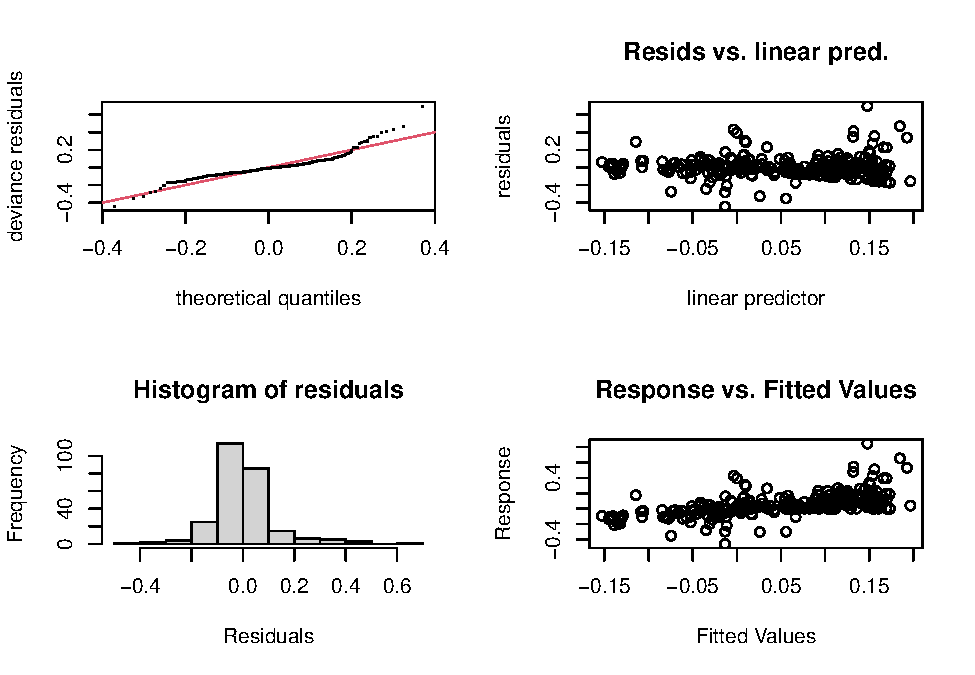
\includegraphics{Forest_and_Water_files/figure-latex/model2b-1.pdf}

\begin{verbatim}
## 
## Method: GCV   Optimizer: magic
## Smoothing parameter selection converged after 8 iterations.
## The RMS GCV score gradient at convergence was 2.042593e-08 .
## The Hessian was positive definite.
## Model rank =  21 / 21 
## 
## Basis dimension (k) checking results. Low p-value (k-index<1) may
## indicate that k is too low, especially if edf is close to k'.
## 
##               k'  edf k-index p-value    
## s(Area_km2) 2.00 1.00    0.97    0.29    
## s(Pa_mm)    2.00 1.25    0.78  <2e-16 ***
## s(From)     2.00 1.00    0.85    0.01 ** 
## s(length)   2.00 1.00    0.90    0.02 *  
## ---
## Signif. codes:  0 '***' 0.001 '**' 0.01 '*' 0.05 '.' 0.1 ' ' 1
\end{verbatim}

\begin{verbatim}
## Warning in eval(predvars, data, env): NaNs produced

## Warning in eval(predvars, data, env): NaNs produced
\end{verbatim}

\begin{verbatim}
## 
## Family: gaussian 
## Link function: identity 
## 
## Formula:
## log10(DeltaQf_perc/100 + 1) ~ DeltaF_perc + s(Area_km2, k = 3) + 
##     s(Pa_mm, k = 3) + s(From, k = 3) + s(length, k = 3) + Precip_data_type + 
##     Assessment_technique + Forest_type + Hydrological_regime
## 
## Parametric coefficients:
##                               Estimate Std. Error t value Pr(>|t|)    
## (Intercept)                 -0.0962315  0.0558563  -1.723   0.0862 .  
## DeltaF_perc                 -0.0008839  0.0001711  -5.165 4.98e-07 ***
## Precip_data_typeOB          -0.0329926  0.0418383  -0.789   0.4311    
## Precip_data_typeSG           0.0595846  0.0474089   1.257   0.2100    
## Assessment_techniqueEA, HM   0.0143199  0.1329271   0.108   0.9143    
## Assessment_techniqueHM       0.0910165  0.0445991   2.041   0.0423 *  
## Assessment_techniquePWE      0.2041286  0.0457201   4.465 1.22e-05 ***
## Assessment_techniquePWE, HM  0.0977846  0.1370941   0.713   0.4764    
## Assessment_techniqueQPW      0.0850446  0.0731186   1.163   0.2459    
## Assessment_techniqueSH       0.1066145  0.0473168   2.253   0.0251 *  
## Forest_typeCF               -0.0029430  0.0268072  -0.110   0.9127    
## Forest_typeMF               -0.0463517  0.0265852  -1.744   0.0825 .  
## Hydrological_regimeSD        0.0111796  0.0319040   0.350   0.7263    
## ---
## Signif. codes:  0 '***' 0.001 '**' 0.01 '*' 0.05 '.' 0.1 ' ' 1
## 
## Approximate significance of smooth terms:
##              edf Ref.df     F p-value  
## s(Area_km2) 1.00  1.000 0.301  0.5839  
## s(Pa_mm)    1.25  1.437 0.640  0.3574  
## s(From)     1.00  1.000 3.194  0.0751 .
## s(length)   1.00  1.000 0.540  0.4631  
## ---
## Signif. codes:  0 '***' 0.001 '**' 0.01 '*' 0.05 '.' 0.1 ' ' 1
## 
## R-sq.(adj) =  0.274   Deviance explained = 31.9%
## GCV = 0.017635  Scale est. = 0.016474  n = 262
\end{verbatim}

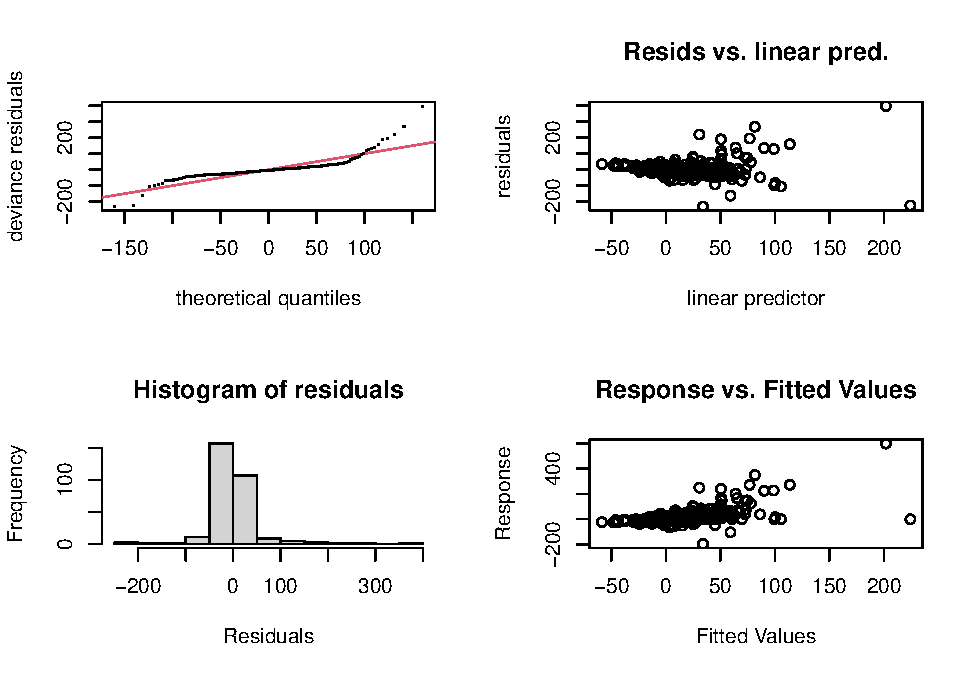
\includegraphics{Forest_and_Water_files/figure-latex/model2c-1.pdf}

\begin{verbatim}
## 
## Method: GCV   Optimizer: magic
## Smoothing parameter selection converged after 8 iterations.
## The RMS GCV score gradient at convergence was 2.042593e-08 .
## The Hessian was positive definite.
## Model rank =  21 / 21 
## 
## Basis dimension (k) checking results. Low p-value (k-index<1) may
## indicate that k is too low, especially if edf is close to k'.
## 
##               k'  edf k-index p-value    
## s(Area_km2) 2.00 1.00    0.97   0.330    
## s(Pa_mm)    2.00 1.25    0.78  <2e-16 ***
## s(From)     2.00 1.00    0.85   0.015 *  
## s(length)   2.00 1.00    0.90   0.095 .  
## ---
## Signif. codes:  0 '***' 0.001 '**' 0.01 '*' 0.05 '.' 0.1 ' ' 1
\end{verbatim}

No evidence of effect of area

\begin{verbatim}
## Warning in eval(predvars, data, env): NaNs produced

## Warning in eval(predvars, data, env): NaNs produced
\end{verbatim}

\begin{verbatim}
## 
## Family: gaussian 
## Link function: identity 
## 
## Formula:
## log10(DeltaQf_perc/100 + 1) ~ DeltaF_perc + log10(Area_km2) + 
##     s(Pa_mm, k = 3) + From + length + Precip_data_type + Assessment_technique + 
##     Forest_type + Hydrological_regime + Latitude + Longitude
## 
## Parametric coefficients:
##                               Estimate Std. Error t value Pr(>|t|)    
## (Intercept)                 -1.2633792  1.1731739  -1.077  0.28260    
## DeltaF_perc                 -0.0010709  0.0001693  -6.324 1.21e-09 ***
## log10(Area_km2)             -0.0106973  0.0079411  -1.347  0.17921    
## From                         0.0006320  0.0005902   1.071  0.28528    
## length                       0.0002020  0.0007979   0.253  0.80032    
## Precip_data_typeOB          -0.0496200  0.0405500  -1.224  0.22226    
## Precip_data_typeSG           0.0379293  0.0474175   0.800  0.42455    
## Assessment_techniqueEA, HM   0.0190552  0.1279391   0.149  0.88173    
## Assessment_techniqueHM       0.0665563  0.0447830   1.486  0.13852    
## Assessment_techniquePWE      0.1335480  0.0529257   2.523  0.01226 *  
## Assessment_techniquePWE, HM  0.0724841  0.1341116   0.540  0.58936    
## Assessment_techniqueQPW      0.0585720  0.0713099   0.821  0.41224    
## Assessment_techniqueSH       0.0649925  0.0482180   1.348  0.17895    
## Forest_typeCF                0.0129954  0.0267350   0.486  0.62735    
## Forest_typeMF               -0.0171200  0.0262238  -0.653  0.51448    
## Hydrological_regimeSD        0.0425574  0.0316727   1.344  0.18031    
## Latitude                    -0.0010038  0.0003307  -3.035  0.00267 ** 
## Longitude                    0.0001756  0.0001025   1.713  0.08803 .  
## ---
## Signif. codes:  0 '***' 0.001 '**' 0.01 '*' 0.05 '.' 0.1 ' ' 1
## 
## Approximate significance of smooth terms:
##            edf Ref.df     F p-value
## s(Pa_mm) 1.004  1.008 1.285   0.256
## 
## R-sq.(adj) =  0.328   Deviance explained = 37.5%
## GCV = 0.016441  Scale est. = 0.015249  n = 262
\end{verbatim}

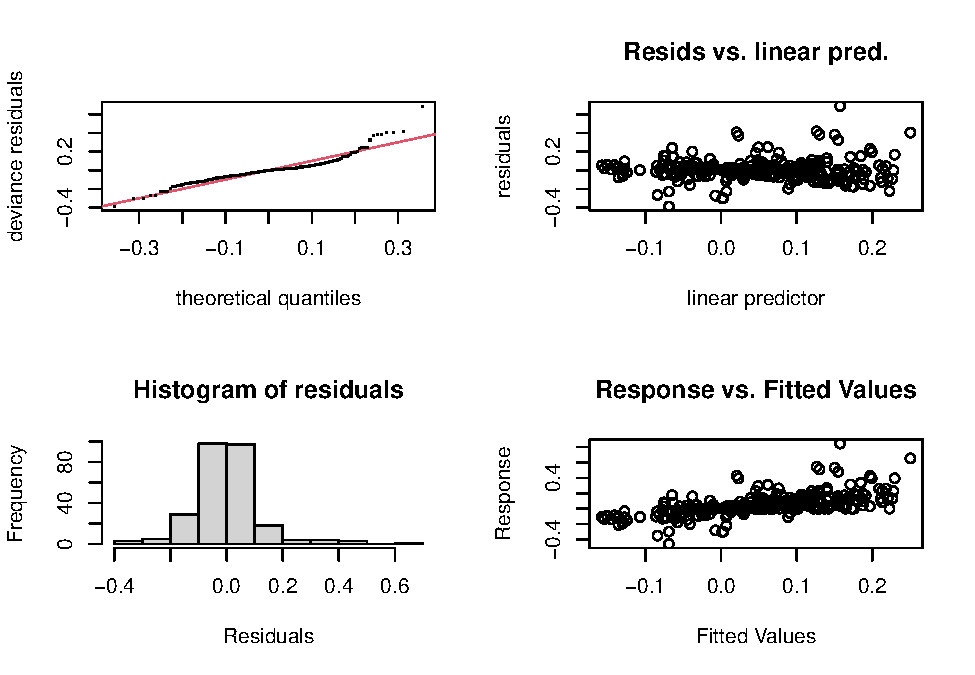
\includegraphics{Forest_and_Water_files/figure-latex/model2d-1.pdf}

\begin{verbatim}
## 
## Method: GCV   Optimizer: magic
## Smoothing parameter selection converged after 5 iterations.
## The RMS GCV score gradient at convergence was 2.648312e-07 .
## The Hessian was positive definite.
## Model rank =  20 / 20 
## 
## Basis dimension (k) checking results. Low p-value (k-index<1) may
## indicate that k is too low, especially if edf is close to k'.
## 
##          k' edf k-index p-value    
## s(Pa_mm)  2   1     0.8  <2e-16 ***
## ---
## Signif. codes:  0 '***' 0.001 '**' 0.01 '*' 0.05 '.' 0.1 ' ' 1
\end{verbatim}

\begin{Shaded}
\begin{Highlighting}[]
\NormalTok{Zhang_all }\OperatorTok
\StringTok{  }\KeywordTok{ggplot}\NormalTok{(}\KeywordTok{aes}\NormalTok{(Assessment_technique,}\KeywordTok{log10}\NormalTok{(Area_km2))) }\OperatorTok{+}\StringTok{ }\KeywordTok{geom_boxplot}\NormalTok{()}
\end{Highlighting}
\end{Shaded}

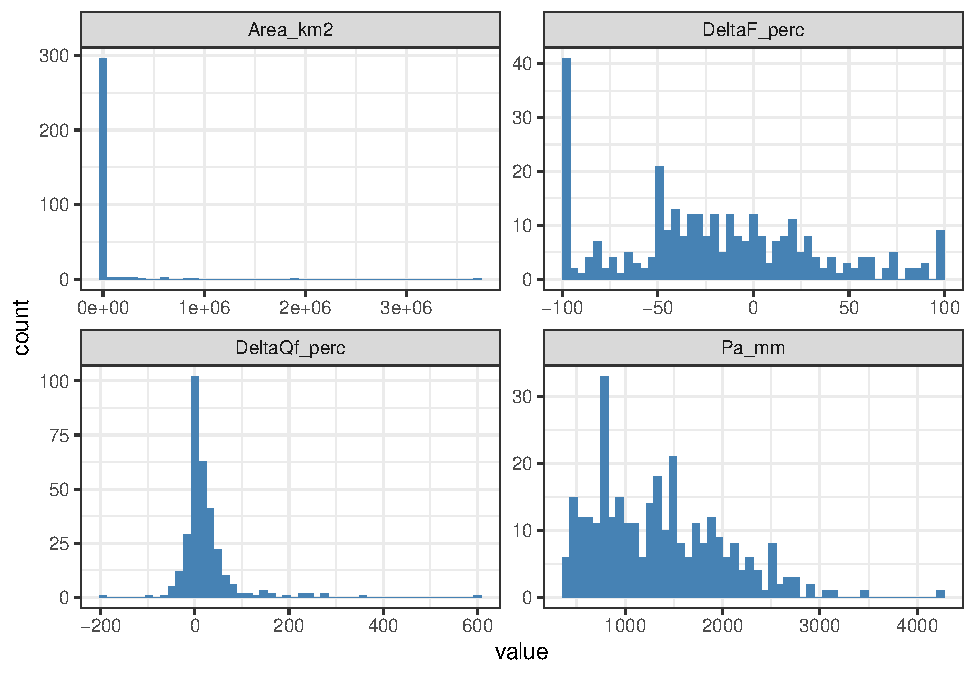
\includegraphics{Forest_and_Water_files/figure-latex/unnamed-chunk-4-1.pdf}

\begin{Shaded}
\begin{Highlighting}[]
\NormalTok{Zhang_all }\OperatorTok
\StringTok{  }\KeywordTok{ggplot}\NormalTok{(}\KeywordTok{aes}\NormalTok{(DeltaF_perc, }\KeywordTok{log10}\NormalTok{(DeltaQf_perc}\OperatorTok{/}\DecValTok{100} \OperatorTok{+}\StringTok{ }\DecValTok{1}\NormalTok{), }\DataTypeTok{colour =}\NormalTok{ Assessment_technique,}\DataTypeTok{size =} \KeywordTok{log10}\NormalTok{(Area_km2))) }\OperatorTok{+}\StringTok{ }\KeywordTok{geom_point}\NormalTok{()}
\end{Highlighting}
\end{Shaded}

\begin{verbatim}
## Warning in FUN(X[[i]], ...): NaNs produced

## Warning in FUN(X[[i]], ...): NaNs produced
\end{verbatim}

\begin{verbatim}
## Warning: Removed 2 rows containing missing values (geom_point).
\end{verbatim}

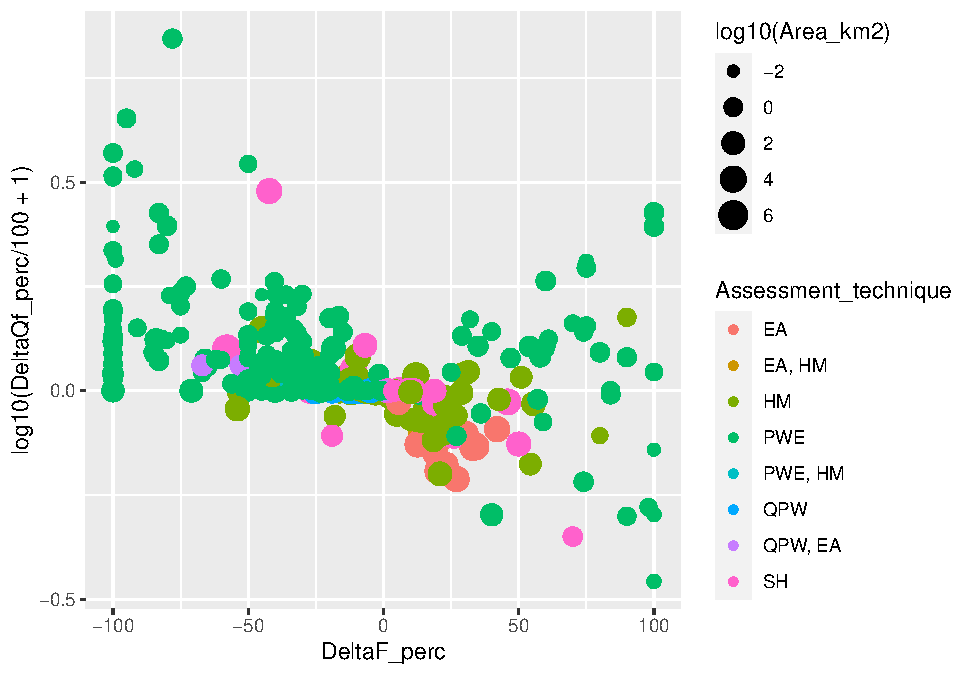
\includegraphics{Forest_and_Water_files/figure-latex/unnamed-chunk-5-1.pdf}

\begin{Shaded}
\begin{Highlighting}[]
\KeywordTok{tiff}\NormalTok{(}\StringTok{"flow_forest_byArea.tiff"}\NormalTok{, }\DataTypeTok{width =} \DecValTok{2000}\NormalTok{, }\DataTypeTok{height =} \DecValTok{1400}\NormalTok{, }\DataTypeTok{res =} \DecValTok{300}\NormalTok{)}
\NormalTok{Zhang_all }\OperatorTok
\StringTok{  }\KeywordTok{ggplot}\NormalTok{(}\KeywordTok{aes}\NormalTok{(DeltaF_perc}\OperatorTok{/}\DecValTok{100}\NormalTok{, (DeltaQf_perc}\OperatorTok{/}\DecValTok{100} \OperatorTok{+}\StringTok{ }\DecValTok{1}\NormalTok{), }\DataTypeTok{colour =}\NormalTok{ Assessment_technique, }\DataTypeTok{size =} \KeywordTok{log10}\NormalTok{(Area_km2))) }\OperatorTok{+}\StringTok{ }\KeywordTok{geom_point}\NormalTok{() }\OperatorTok{+}
\StringTok{  }\KeywordTok{theme_bw}\NormalTok{() }\OperatorTok{+}\StringTok{ }\KeywordTok{ylab}\NormalTok{(}\StringTok{"log10 (fractional change in flow + 1)"}\NormalTok{) }\OperatorTok{+}
\StringTok{  }\KeywordTok{xlab}\NormalTok{(}\StringTok{"fractional change in forestry"}\NormalTok{) }\OperatorTok{+}\StringTok{ }\KeywordTok{scale_y_log10}\NormalTok{() }\OperatorTok{+}\StringTok{ }\KeywordTok{scale_size_continuous}\NormalTok{(}\DataTypeTok{name =} \StringTok{"log10 Area in km2"}\NormalTok{) }\OperatorTok{+}
\StringTok{  }\KeywordTok{scale_colour_discrete}\NormalTok{(}\DataTypeTok{name =} \StringTok{"Assessment Technique"}\NormalTok{)}
\end{Highlighting}
\end{Shaded}

\begin{verbatim}
## Warning in self$trans$transform(x): NaNs produced
\end{verbatim}

\begin{verbatim}
## Warning: Transformation introduced infinite values in continuous y-axis
\end{verbatim}

\begin{verbatim}
## Warning: Removed 2 rows containing missing values (geom_point).
\end{verbatim}

\begin{Shaded}
\begin{Highlighting}[]
\KeywordTok{dev.off}\NormalTok{()}
\end{Highlighting}
\end{Shaded}

\begin{verbatim}
## pdf 
##   2
\end{verbatim}

\begin{Shaded}
\begin{Highlighting}[]
\NormalTok{Zhang_all }\OperatorTok
\StringTok{  }\KeywordTok{ggplot}\NormalTok{(}\KeywordTok{aes}\NormalTok{(Latitude, }\KeywordTok{log10}\NormalTok{(DeltaQf_perc}\OperatorTok{/}\DecValTok{100} \OperatorTok{+}\StringTok{ }\DecValTok{1}\NormalTok{), }\DataTypeTok{colour =}\NormalTok{ DeltaF_perc,}\DataTypeTok{size =} \KeywordTok{log10}\NormalTok{(Area_km2))) }\OperatorTok{+}\StringTok{ }\KeywordTok{geom_point}\NormalTok{()}
\end{Highlighting}
\end{Shaded}

\begin{verbatim}
## Warning in FUN(X[[i]], ...): NaNs produced

## Warning in FUN(X[[i]], ...): NaNs produced
\end{verbatim}

\begin{verbatim}
## Warning: Removed 8 rows containing missing values (geom_point).
\end{verbatim}

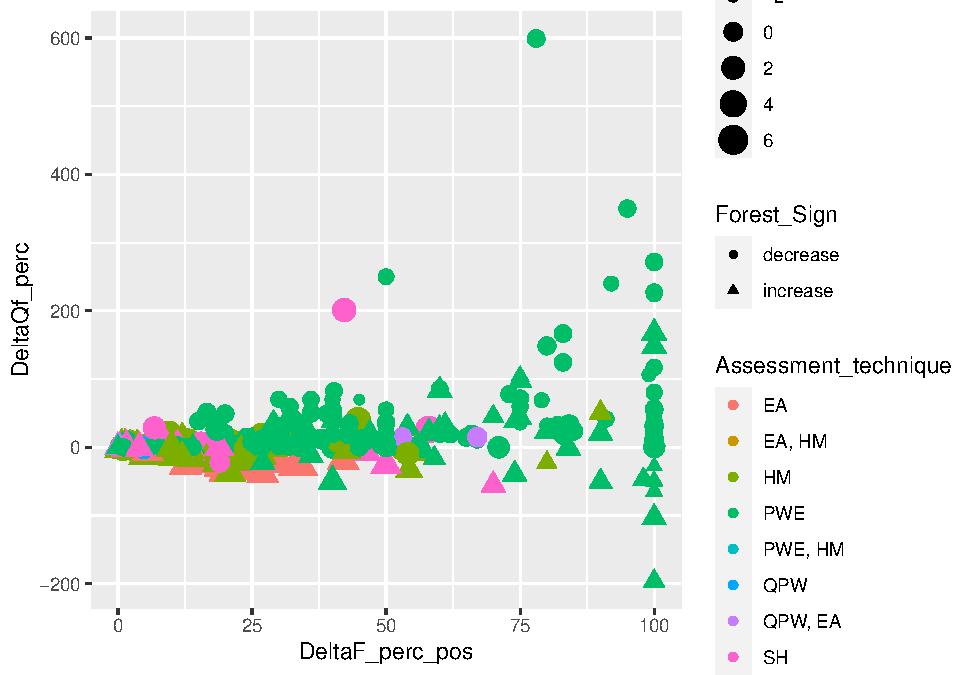
\includegraphics{Forest_and_Water_files/figure-latex/unnamed-chunk-7-1.pdf}

Check the size distribition of the catchments

\begin{Shaded}
\begin{Highlighting}[]
\NormalTok{Zhang_all }\OperatorTok
\StringTok{  }\KeywordTok{ggplot}\NormalTok{(}\KeywordTok{aes}\NormalTok{(Area_km2)) }\OperatorTok{+}\StringTok{ }\KeywordTok{geom_histogram}\NormalTok{(}\DataTypeTok{fill=}\StringTok{"blue"}\NormalTok{, }\DataTypeTok{bins =}\DecValTok{50}\NormalTok{) }\OperatorTok{+}
\StringTok{  }\KeywordTok{scale_x_log10}\NormalTok{()}
\end{Highlighting}
\end{Shaded}

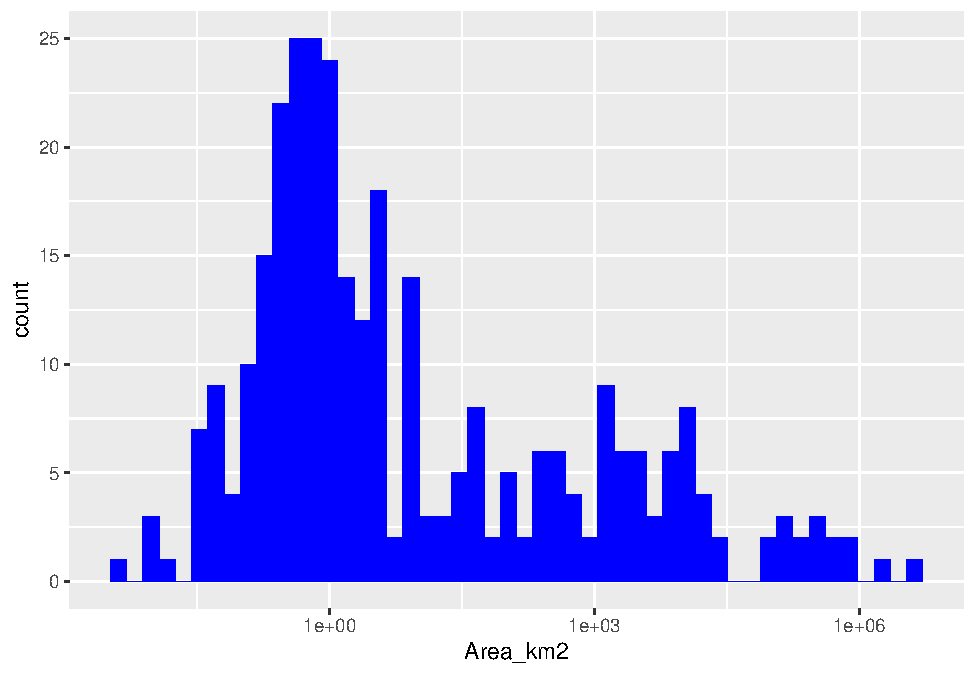
\includegraphics{Forest_and_Water_files/figure-latex/unnamed-chunk-8-1.pdf}

\begin{Shaded}
\begin{Highlighting}[]
\NormalTok{total <-}\StringTok{ }\KeywordTok{nrow}\NormalTok{(Zhang_all)}
\KeywordTok{length}\NormalTok{(Zhang_all}\OperatorTok{$}\NormalTok{Area_km2[Zhang_all}\OperatorTok{$}\NormalTok{Area_km2}\OperatorTok{<}\DecValTok{10}\NormalTok{])}\OperatorTok{/}\NormalTok{total}
\end{Highlighting}
\end{Shaded}

\begin{verbatim}
## [1] 0.6570513
\end{verbatim}

\hypertarget{references}{%
\section*{References}\label{references}}
\addcontentsline{toc}{section}{References}

\hypertarget{refs}{}
\leavevmode\hypertarget{ref-andreassian2004}{}%
Andréassian, V., 2004. Waters and forests: From historical controversy
to scientific debate. Journal of Hydrology 291, 1--27.
doi:\href{https://doi.org/https://doi.org/10.1016/j.jhydrol.2003.12.015}{https://doi.org/10.1016/j.jhydrol.2003.12.015}

\leavevmode\hypertarget{ref-borg1988}{}%
Borg, H., Bell, R.W., Loh, I.C., 1988. Streamflow and stream salinity in
a small water supply catchment in southwest western australia after
reforestation. Journal of Hydrology 103, 323--333.
doi:\href{https://doi.org/https://doi.org/10.1016/0022-1694(88)90141-2}{https://doi.org/10.1016/0022-1694(88)90141-2}

\leavevmode\hypertarget{ref-hewlett1984}{}%
Bosch, J.M., Hewlett, J.D., 1982. A review of catchment experiments to
determine the effect of vegetation changes on water yield and
evapotranspiration. Journal of Hydrology 55, 3--23.

\leavevmode\hypertarget{ref-brown2013}{}%
Brown, A.E., Western, A.W., McMahon, T.A., Zhang, L., 2013. Impact of
forest cover changes on annual streamflow and flow duration curves.
Journal of Hydrology 483, 39--50.
doi:\href{https://doi.org/http://dx.doi.org/10.1016/j.jhydrol.2012.12.031}{http://dx.doi.org/10.1016/j.jhydrol.2012.12.031}

\leavevmode\hypertarget{ref-brown2005}{}%
Brown, A.E., Zhang, L., McMahon, T.A., Western, A.W., Vertessy, R.A.,
2005. A review of paired catchment studies for determining changes in
water yield resulting from alterations in vegetation. Journal of
Hydrology 310, 28--61.

\leavevmode\hypertarget{ref-cosandey2005}{}%
Cosandey, C., Andréassian, V., Martin, C., Didon-Lescot, J.F., Lavabre,
J., Folton, N., Mathys, N., Richard, D., 2005. The hydrological impact
of the mediterranean forest: A review of french research. Journal of
Hydrology 301, 235--249.
doi:\href{https://doi.org/https://doi.org/10.1016/j.jhydrol.2004.06.040}{https://doi.org/10.1016/j.jhydrol.2004.06.040}

\leavevmode\hypertarget{ref-filoso2017}{}%
Filoso, S., Bezerra, M.O., Weiss, K.C.B., Palmer, M.A., 2017. Impacts of
forest restoration on water yield: A systematic review. PLOS ONE 12,
e0183210.
doi:\href{https://doi.org/10.1371/journal.pone.0183210}{10.1371/journal.pone.0183210}

\leavevmode\hypertarget{ref-jackson2005}{}%
Jackson, R.B., Jobbagy, E.G., Avissar, R., Roy, S.B., Barrett, D.J.,
Cook, C.W., Farley, K.A., Maitre, D.C. le, McCarl, B.A., Murray, B.C.,
2005. Trading water for carbon with biological carbon sequestration.
Science 310, 1944--1947.
doi:\href{https://doi.org/10.1126/science.1119282}{10.1126/science.1119282}

\leavevmode\hypertarget{ref-pena-arancibia2012}{}%
Peña-Arancibia, J.L., Dijk, A.I.J.M. van, Guerschman, J.P., Mulligan,
M., Bruijnzeel, L.A., McVicar, T.R., 2012. Detecting changes in
streamflow after partial woodland clearing in two large catchments in
the seasonal tropics. Journal of Hydrology 416-417, 60--71.
doi:\href{https://doi.org/https://doi.org/10.1016/j.jhydrol.2011.11.036}{https://doi.org/10.1016/j.jhydrol.2011.11.036}

\leavevmode\hypertarget{ref-rodriguez2010}{}%
Rodriguez, D.A., Tomasella, J., Linhares, C., 2010. Is the forest
conversion to pasture affecting the hydrological response of amazonian
catchments? Signals in the ji-paraná basin. Hydrological Processes 24,
1254--1269.
doi:\href{https://doi.org/https://doi.org/10.1002/hyp.7586}{https://doi.org/10.1002/hyp.7586}

\leavevmode\hypertarget{ref-ruprechtetal1991}{}%
Ruprecht, J.K., Schofield, N.J., Crombie, D.S., Vertessy, R.A.,
Stoneman, G.L., 1991. Early hydrological response to intense forest
thinning in southwestern australia. Journal of Hydrology 127, 261--277.
doi:\href{https://doi.org/https://doi.org/10.1016/0022-1694(91)90118-2}{https://doi.org/10.1016/0022-1694(91)90118-2}

\leavevmode\hypertarget{ref-thornton2007}{}%
Thornton, C.M., Cowie, B.A., Freebairn, D.M., Playford, C.L., 2007. The
brigalow catchment study: II*. Clearing brigalow (acacia harpophylla)
for cropping or pasture increases runoff. Australian Journal of Soil
Research 45, 496--511.
doi:\href{https://doi.org/doi:10.1071/SR07064}{doi:10.1071/SR07064}

\leavevmode\hypertarget{ref-wood2006}{}%
Wood, S., 2006. Generalized additive models: An introduction with r. CRC
Press, Boca Raton, FL.

\leavevmode\hypertarget{ref-zhang2011}{}%
Zhang, L., Zhao, F., Chen, Y., Dixon, R.N.M., 2011. Estimating effects
of plantation expansion and climate variability on streamflow for
catchments in australia. Water Resources Research 47, W12539.
doi:\href{https://doi.org/10.1029/2011wr010711}{10.1029/2011wr010711}

\leavevmode\hypertarget{ref-zhang2017}{}%
Zhang, M., Liu, N., Harper, R., Li, Q., Liu, K., Wei, X., Ning, D., Hou,
Y., Liu, S., 2017. A global review on hydrological responses to forest
change across multiple spatial scales: Importance of scale, climate,
forest type and hydrological regime. Journal of Hydrology 546, 44--59.
doi:\href{https://doi.org/https://doi.org/10.1016/j.jhydrol.2016.12.040}{https://doi.org/10.1016/j.jhydrol.2016.12.040}

\leavevmode\hypertarget{ref-zhao2010}{}%
Zhao, F., Zhang, L., Xu, Z., Scott, D.F., 2010. Evaluation of methods
for estimating the effects of vegetation change and climate variability
on streamflow. Water Resources Research 46, W03505.
doi:\href{https://doi.org/10.1029/2009wr007702}{10.1029/2009wr007702}

\leavevmode\hypertarget{ref-zhou2015}{}%
Zhou, G., Wei, X., Chen, X., Zhou, P., Liu, X., Xiao, Y., Sun, G.,
Scott, D.F., Zhou, S., Han, L., Su, Y., 2015. Global pattern for the
effect of climate and land cover on water yield. Nature Communications
6, 5918.
doi:\href{https://doi.org/10.1038/ncomms6918}{10.1038/ncomms6918}

\leavevmode\hypertarget{ref-zhou2010}{}%
Zhou, G., Wei, X., Luo, Y., Zhang, M., Li, Y., Qiao, Y., Liu, H., Wang,
C., 2010. Forest recovery and river discharge at the regional scale of
guangdong province, china. Water Resources Research 46.
doi:\href{https://doi.org/https://doi.org/10.1029/2009WR008829}{https://doi.org/10.1029/2009WR008829}


\end{document}


